% Last update/Última versão: 11/Sep/2016
%%%%%%%%%%%%%%%%%%%%%%%%%%%%%%%%%%%%%%%%%%%%%%%%%%%%%%%%%%%%%%%%%%%%%%
%=====================================================================
% 							Pacotes Fundamentais
%=====================================================================
\documentclass[
% -- op\c{c}\~{o}es da classe memoir --
12pt,				% tamanho da fonte
openright,			% cap\'{\i}tulos come\c{c}am em p\'{a}g \'{\i}mpar (insere p\'{a}gina vazia caso preciso)
oneside,			% para impress\~{a}o em verso e anverso. Oposto a oneside
a4paper,		% tamanho do papel.
% -- op\c{c}\~{o}es da classe abntex2 --
%chapter=TITLE,		% t\'{\i}tulos de cap\'{\i}tulos convertidos em letras mai\'{u}sculas
%section=TITLE,		% t\'{\i}tulos de se\c{c}\~{o}es convertidos em letras mai\'{u}sculas
%subsection=TITLE,	% t\'{\i}tulos de subse\c{c}\~{o}es convertidos em letras mai\'{u}sculas
%subsubsection=TITLE,% t\'{\i}tulos de subsubse\c{c}\~{o}es convertidos em letras mai\'{u}sculas
% -- op\c{c}\~{o}es do pacote babel --
english,			% idioma adicional para hifeniza\c{c}\~{a}o
%french,			% idioma adicional para hifeniza\c{c}\~{a}o
%spanish,			% idioma adicional para hifeniza\c{c}\~{a}o
brazil,				% o \'{u}ltimo idioma \'{e} o principal do documento
%sumario=tradicional,
]{article}
\usepackage[a4paper, right = 1.5cm, left = 3.5cm, top = 3 cm, bottom = 2cm]{geometry}
\usepackage[utf8]{inputenc}
\usepackage[english,portuguese]{babel}
\usepackage[myheadings]{fullpage}
\usepackage[T1]{fontenc}
\usepackage{fancyhdr}
\usepackage{graphicx, setspace}
\usepackage{sectsty}
\usepackage{url}
\usepackage{mathptmx} %% Para times
\usepackage{comment}
\usepackage{multirow}
\usepackage[table,xcdraw]{xcolor}
\usepackage{enumitem}
\usepackage{blindtext}
\usepackage{float}
\usepackage[bottom]{footmisc}
\usepackage{pdfpages}
\usepackage{caption}
\usepackage{csquotes}


%=====================================================================
% 							Pacotes Bibliográficos
%=====================================================================

\usepackage[backend=biber,
	style = abnt,%
	noslsn, %
	extrayear, %
	uniquename=init,% 
	giveninits, %
	justify, %
	sccite,% 
	scbib, %
	repeattitles, %
	maxcitenames=3]{biblatex}
\addbibresource{Bib_FAPESP_Mestrado.bib}


%=====================================================================
% 							Comandos específicos da FAPESP
%=====================================================================
\newcommand{\HRule}[1]{\rule{\linewidth}{#1}}
\onehalfspacing
\setcounter{tocdepth}{3}
\setcounter{secnumdepth}{3}

\newcommand{\titulo}[1]{\def\meuTitulo{#1}}
\newcommand{\tituloIngles}[1]{\def\meuTituloIngles{#1}}
\newcommand{\numFAPESP}[1]{\def\numFAP{#1}}
\newcommand{\tipoRelatorio}[1]{\def\tipoRelat{#1 }} %o espaço depois do #1 é importante
\newcommand{\autor}[1]{\def\nomeAutor{#1}}
\newcommand{\cidade}[1]{\def\nomeCidade{#1}}
\newcommand{\universidade}[1]{\def\nomeUniversidade{#1}}
\newcommand{\faculdade}[1]{\def\nomeFaculdade{#1}}
\newcommand{\periodoVigencia}[1]{\def\periodVig{#1}}
\newcommand{\periodoRelatorio}[1]{\def\periodRelat{#1}}
\author{}
\date{}

\newcommand{\Figure}[1]{Figura~\ref{fig:#1}}
\newcommand{\Table}[1] {Tabela~\ref{#1}}
\newcommand{\Equation}[1] {Equa\c{c}\~ao~\ref{#1}}
\newcommand{\addFigure}[3] { %Parametros scale, fig_name, caption 
    \begin{figure}[!hbt]
      \centering
      \includegraphics[scale=#1]{figures/#2}
      \caption{#3}\label{fig:#2}
    \end{figure}
}

\newcommand{\geraTitulo}{
\clearpage
\begin{titlepage}
  \begin{center}
      \vspace*{-3cm}
      { \setstretch{.5} 
        \textsc{\nomeUniversidade} \\
        \HRule{.2pt}\\
        \textsc{\nomeFaculdade}
      }

      \vspace{5.5cm}

      \Large \textbf{\textsc{\meuTitulo}}
	  \HRule{1.5pt} \\ [0.5cm]
      \linespread{1}
      \large Relatório Científico \tipoRelat do Projeto de Auxílio à Pesquisa Regular, fomentado pela Fundação de Amparo à Pesquisa do Estado de São Paulo. \\ 
  	   \HRule{1.5pt} \\ [0.5cm]
       Projeto FAPESP \texttt{\#\numFAP}
       \\ [0.1cm]
       Pesquisador Responsável: \nomeAutor
       
       \vfill
       
       {\normalsize  \nomeCidade, \today}
\end{center}
\end{titlepage}
}

\usepackage{titlesec}
\titleformat{\chapter}{\normalfont\LARGE\bfseries}{\thechapter}{1em}{}
\titlespacing*{\chapter}{0pt}{3.5ex plus 1ex minus .2ex}{2.3ex plus .2ex}

%----------------------------------------------------------------------
% HEADER & FOOTER
%----------------------------------------------------------------------
\pagestyle{fancy}
\fancyhf{} % Limpa todos os campos de header and footer fields
%\setlength\headheight{15pt}
\renewcommand{\headrulewidth}{0pt}
%\fancyhead[R]{Anglia Ruskin University} 
\fancyfoot[R]{\thepage}%of \pageref{LastPage}}

\addto\captionsportuguese{\renewcommand{\contentsname}{Sumário}}
\addto\captionsportuguese{\renewcommand{\bibname}{Referências bibliográficas}}

%------
% Resumo e Abstract
%------
\newcommand{\Resumo}[1]{
   \begin{otherlanguage}{portuguese}
       \addcontentsline{toc}{chapter}{Resumo}
       \begin{abstract} \thispagestyle{plain} \setcounter{page}{2}
          #1
        \end{abstract}
   \end{otherlanguage} 
} %end \Resumo

\newcommand{\Abstract}[1]{
   \begin{otherlanguage}{english}
      \addcontentsline{toc}{chapter}{Abstract}
      \begin{abstract} \thispagestyle{plain} \setcounter{page}{3}
       #1
      \end{abstract}    
    \end{otherlanguage} 
} %end \abstract

%------
% Folha de rosto
%------
\newcommand{\folhaDeRosto}{
   \chapter*{Informações Gerais do Projeto}
   \addcontentsline{toc}{chapter}{Informações Gerais do Projeto}
   \begin{itemize}
      \item Título do projeto: 
            \begin{itemize}\item[] \textbf{\meuTitulo} \end{itemize}
      \item Nome do pesquisador responsável: 
            \begin{itemize}\item[]\textbf{\nomeAutor}\end{itemize}
      \item Instituição sede do projeto: 
            \begin{itemize}
               \item[]\textbf{\nomeFaculdade \ da \nomeUniversidade} 
            \end{itemize}
      \item Equipe de pesquisa:
            \begin{itemize}
               \item[]\textbf{\nomeAutor} 
            \end{itemize}
       \item Número do projeto de pesquisa:
            \begin{itemize}
               \item[]\textbf{\numFAP} 
            \end{itemize}
       \item Período de vigência:
            \begin{itemize}
               \item[]\textbf{\periodRelat} 
            \end{itemize}
       \item Período coberto por este relatório científico:
            \begin{itemize}
               \item[]\textbf{\periodVig} 
            \end{itemize}
   \end{itemize}
   \clearpage
}
%=====================================================================
% 							Outros Pacotes
%=====================================================================
\usepackage[colorinlistoftodos]{todonotes}
\usepackage{subfigure}
\usepackage{setspace}

%=====================================================================
% 							Página de título e folha de rosto
%=====================================================================
%-----
% Página de título
% Observação: As definições que aparecem a seguir comporão a
%             página de título e a folha de rosto.
%-----
%% Define o nome da universidade onde o projeto foi desenvolvido.
\universidade{Universidade Estadual de Campinas}
%
%% Define o nome da faculdade onde o projeto foi desenvolvido.
\faculdade{Instituto de Economia}
%
%% Define o título do projeto.
\titulo{Distribuição de renda, crédito e crescimento: 
	Uma análise a partir da teoria monetária da distribuição 
	para o caso brasileiro recente (2003-2014)}
%
%% Define o tipo de relatório Anual ou Final.
% \tipoRelatorio{Final}
%
%% Define o autor do relatório.
\autor{Gabriel Petrini da Silveira}
%
%% Define o número do projeto.
%\numFAPESP{NÚMERO}
%
%% Define o período da vigência do Projeto.
%\periodoVigencia{01/agosto/2018 a 01/janeiro/2020}
%
%% Define o período coberto pelo relatório.
%\periodoRelatorio{01/junho/2015 a 30/maio/2017}
%
%% Define a cidade onde o projeto foi desenvolvido.
\cidade{Campinas}

\begin{document}
%=====================================================================
% 							Numeração pré-textual
%=====================================================================
\pagenumbering{roman}
%=====================================================================
% 							Folha de título
%=====================================================================
\geraTitulo
%=====================================================================
% 							Folha de rosto
%=====================================================================
% Gera a folha de rosto.
\folhaDeRosto
%=====================================================================
% 							Resumo
%=====================================================================
\begin{abstract}
	em português aqui
\end{abstract}
%=====================================================================
% 							Abstract
%=====================================================================
\folhaDeRostoEN

{
	\selectlanguage{english}
	\begin{abstract}
		insert here
	\end{abstract}
}
\clearpage
%=====================================================================
% 							Sumário
%=====================================================================
%\tableofcontents
%\thispagestyle{empty}
%\clearpage
%=====================================================================
% 							Numeração textual
%=====================================================================
\pagenumbering{arabic}

%=====================================================================
% 							Formatação título seção
%=====================================================================
\sectionfont{\scshape}

%=====================================================================
% 							Corpo de texto
%=====================================================================
%\listoftodos
\doublespacing
\begingroup
\let\clearpage\relax
Uma das fronteiras da pesquisa empírica acerca da literatura de crescimento liderado pela demanda é aquela que enfatiza a importância dos gastos autônomos não criadores de capacidade produtiva ao setor privado. \textcite{freitas_pattern_2013}, por exemplo, decompõem o crescimento da economia brasileira mostrando o papel desses gastos para os anos de  1970 a 2005. \textcite{braga_investment_2018} conclui que os gastos improdutivos lideram o crescimento e que o investimento produtivo acompanha a tendência desses gastos, ao analisar o Brasil no período 1962-2015. Para o caso norte-americano, \textcite{girardi_long-run_2016} encontram evidências de que os gastos autônomos causam efeitos de longo prazo na taxa de crescimento enquanto \textcite{girardi_autonomous_2018} complementam com 20 países da OCDE. No entanto, por mais que exista uma literatura crescente sobre o papel dos gastos autônomos no crescimento econômico, ainda há poucos trabalhos que enfatizam a importância do investimento residencial em particular. 
%Com a notória exceção de \textcite{green_follow_1997} e \textcite{leamer_housing_2007}, a maioria desses trabalhos foi publicada após a crise dos \textit{subprime} de 2008 --- que evidenciou a relevância deste gasto para a dinâmica da economia norte-americana.

Desse modo, enquanto o capítulo anterior elegeu o modelo teórico mais adequado para atender os objetivos desta pesquisa, o presente capítulo pretende fornecer a base empírica dessa discussão. Portanto, busca-se uma forma de modelar a taxa de crescimento do investimento residencial que será utilizada nas simulações do capítulo seguinte. 
Cabe frisar que essa análise se restringe ao caso norte-americano no pós-desregulamentação bancária dos anos 80, especialmente após 1991. A razão deste recorte temporal decorre tanto da estagnação salarial observada desde a década passada \cites{mian_house_2011}{teixeira_uma_2011} que implicou na intensa substituição de salário por empréstimos \cite{barba_rising_2009} quanto da crescente participação das hipotecas no balanço patrimonial dos bancos \cite{jorda_great_2014} bem como mudanças regulatórias que reduziram as restrições ao acesso de crédito no mercado imobiliário no pós-crise dos \textit{savings and loans} \cites{linneman_impacts_1989}{duca_empirical_1991}{federal_deposit_insurance_corporation_savings_1997}. 

Compreendidos os objetivos deste capítulo, a seção seguinte irá avaliar os estudos empíricos que incorporam gastos autônomos não criadores de capacidade dando especial ênfase aqueles que utilizam o modelo do supermultiplicador sraffiano (SSM) e, portanto, complementar a discussão teórica realizada no capítulo anterior. 
Em seguida, cabe a seção \ref{Secao_Residencial} destacar a importância do investimento residencial para a dinâmica norte-americana. Além disso, nessa mesma seção são pontuadas as formas com que a literatura trata do tema bem como selecionar a proposta mais adequada e compatível com o SSM. 
Adiante, na seção \ref{Modelo_empirico}, é estimado um modelo  para averiguar os determinantes do investimento residencial para então comparar com os resultados obtidos com os da literatura. Por fim, a seção \ref{Conclucao_Empirica} apresenta as conclusões.
\section{Objetivos}\label{OBJ}

\begin{description}
	\item[Objetivo geral] Investigar os arranjos institucionais do mercado imobiliário e de crédito dos países da OCDE e investigar as implicações sobre o investimento residencial e contrastá-las com o caso norte-americano
	\item[Objetivos específicos] {\color{white} Texto em branco para espaçamento}
	\begin{itemize}
		\item Examinar o processo de ``hipotecarização'' destacado por \textcite{jorda_great_2014};
		\item Comparar o caso norte-americano com os demais países da OCDE;
		\item Testar a aplicabilidade da taxa própria de juros dos imóveis desenvolvida por \textcite{teixeira_crescimento_2015} para os países da OCDE; 
		\item Detectar os principais determinantes macroeconômicos do investimento residencial por meio de um modelo de dados em painel com auxílio da base de dados desenvolvida por \textcite{jorda_great_2014};
		\item Construir um modelo SFC com supermultiplicador sraffiano cujo gasto autônomo é o investimento residencial e replicar as referidas características institucionais do mercados de crédito e imobiliário.
	\end{itemize}
\end{description}


Para atender estes objetivos, a pesquisa proposta será dividida em três frentes cada qual com seu respectivo capítulo.
A primeira delas trata da inserção e contextualização do investimento residencial em processos mais estruturais como a financeirização em contraposição a ``hipotecarização''. Para isso, serão analisadas as especificidades dos países em questão no que diz respeito ao mercado imobiliário e sua conexão com o mercado de crédito bem como a regulação de preços dos imóveis. Em outras palavras, caberá a este capítulo investigar o quão destoante é o caso norte-americano frente aos demais, com especial ênfase ao caso alemão. Compreendidas as especificidades institucionais de cada país, o capítulo seguinte irá analisar os determinantes do investimento residencial por meio de um modelo de dados em panel. Com isso, esses dois capítulos fornecem o embasamento qualitativo e quantitativo para o modelo teórico que será desenvolvido no terceiro capítulo da tese. A partir da metodologia \textit{Stock-Flow Consistent} (SFC), serão testados os diferentes arranjos institucionais destacados no capítulo primeiro bem como os determinantes do investimento residencial reportados no capítulo segundo e, assim, conectar com a literatura do supermultiplicador sraffiano. Sendo assim, cabe a seção seguinte esclarecer as etapas da metodologia SFC.

\section{Justificativa}\label{Just}
A discussão em torno da distribuição de renda tem ganhado destaque na literatura econômica e apresentado resultados relevantes no que diz respeito às teorias de crescimento. Estudos recentes analisando a economia norte-americana reportam a importância da distribuição de renda na determinação da dinâmica econômica. \textcite{grossmann-wirth_role_2018}, por exemplo, explicam a lenta recuperação dos EUA à partir da redução do consumo das famílias no pós Grande Recessão. Partindo da análise dos fluxos das dívidas familiares, os autores concluem  que o consumo privado não tem a capacidade de se basear no endividamento tal como antes.\todo[color=gray!40]{Revisto}

O endividamento das famílias norte-americanas mencionado acima pode ser entendido à partir da piora na distribuição de renda, ou ainda, da redistribuição funcional da renda à favor dos lucros. \textcite{barba_rising_2009} argumentam que o arranjo composto por manutenção do padrão de consumo relativo\footnote{Padrão de consumo relativo no sentido aspiracional, ou seja, manter um nível de vida em linha com as famílias em situação financeira semelhante e, ao mesmo tempo, modernizar os bens consumidos tal como as classes melhor remuneradas. \textcite{barba_rising_2009} lançam mão desta noção a partir do conceito de consumo conspícuo de \textcite{veblen_teoria_1965}.} e estagnação salarial fez com que as famílias dos estratos de renda mais baixos se endividassem\todo[]{Reformular Passividade familias}. Com isso, houve um processo de substituição das rendas do trabalho por empréstimos, permitindo que o crescimento econômico se baseasse no consumo privado. Como contrapartida, verificou-se uma redução significativa da poupança privada, ou em outros termos, uma diminuição dos saldos financeiros líquidos do setor privado \cite{godley_seven_1999}. 

Esta interpretação mostra, portanto, que o endividamento crescente das famílias é resultado tanto de mudanças persistentes na distribuição de renda quanto da elevada desigualdade. Dessa forma, houve um descolamento entre dispêndio e salários de tal modo que foram necessárias outras fontes de recursos para prover esta sofisticação do consumo.
Assim, fica evidente a importância dinâmica do crédito privado que, ao permitir um padrão de crescimento pautado no consumo, tornou possível que  os trabalhadores gastassem muito além dos seus rendimentos, ou melhor, aquilo que não ganham \cite{serrano_trabajadores_2008}. \todo[color=blue!40]{Non-sectur?}

 
Dessa forma, a Grande Recessão mostrou como o aumento do serviço da dívida privada em termos da renda disponível pode gerar processos dinamicamente insustentáveis quando acompanhado de uma piora da distribuição de renda.
Nesses termos, a experiência norte-americana recente sugere que o endividamento das famílias pode ter resultados macroeconômicos distintos no curto, médio e longo prazo. \todo[color=blue!40]{Non-sectur?}
Sendo assim, fica mais do que evidente a importância de se discutir as relações entre distribuição de renda e crescimento.

No entanto, apesar da relevância dos resultados apresentados anteriormente, há muito o que ser explorado e com isso assinala-se a relevância deste projeto\footnote{\textcite{szymborska_household_2018}, por exemplo, afirma que pouco se sabe os tipos de riqueza responsáveis pela melhora (ou piora) da distribuição de renda das famílias. Partindo dos dados do \textit{Survey of Consumer Finances}, conclui que diferentes formas de riqueza afetam a distribuição de renda de maneira distinta. Nesses termos, fica explicito que por mais que este tema seja bastante debatido, existem muitas lacunas a serem preenchidas.}. 
Além disso, por mais distinto que seja o objeto de análise em questão, há muito do se que incorporar dos estudos referentes à outros países. \todo[color=blue!40]{Frase jogada?} 

As diferenças, por sua vez, também podem ser fontes adicionais para inspiração de pesquisas futuras. Não é preciso adentrar nas especificidades institucionais para evidenciar as distinções entre o caso norte-americano e o brasileiro. Neste caso em particular, observa-se que o aumento do endividamento das famílias norte-americanas esteve concentrado nos menores estratos de renda. Partindo desta constatação, \textcite{stockhammer_rising_2015} conclui que a Grande Recessão é resultado tanto da desregulamentação financeira quanto dos efeitos macroeconômicos da desigualdade. O caso brasileiro, em seu turno, possui nuances significativas em que as políticas macroeconômicas redistributivas possibilitaram uma melhora nos menores estratos enquanto pesquisas recentes sugerem um acirramento da concentração entre os mais ricos no mesmo período \cite{medeiros_upper_2015}.


Diante disso, propõe-se investigar como a modernização do padrão de consumo das famílias acompanhada da presença crescente do crédito ao consumidor teve implicações relvantes sobre o crescimento. \todo{Reformular}
Desta forma, a principal justificativa desta pesquisa é a importância dos efeitos e especificidades das mudanças relativas nas parcelas de renda no período recente (2003-2014) para a dinâmica econômica brasileira. Em especial, destaca-se o aumento do endividamento privado \cite{ribeiro_o_2016} junto  da ascensão tanto de uma cultura \textit{política} do consumo quanto uma democratização pelo consumo \todo{Rep Consumo} \cite{fontenelle_alcances_2016}. 

É digno de nota que, com a publicação da portaria \todo[color=green!40]{Ver portaria},
% TODO encontrar número da portaria
serão divulgados relatórios anuais (à partir de 2014) referentes aos dados provenientes do Imposto sobre a Renda da Pessoa Física (IRPF) que trarão não apenas fontes adicionais para se estudar distribuição pessoal da renda como também uma base de comparação entre diferentes levantamentos domiciliares (\textit{i.e.} PNAD, Censo e POF\footnote{Em \textcite{souza_distribuicao_2015}, são apresentadas as diferenças entre essas pesquisa em termos da distribuição de renda. O autor conclui que existe um certo padrão entre as discrepâncias mesmo após uma harmonização \textit{ex post} das séries. A PNAD, em especial, apresenta um teor mais igualitário em que a renda dos mais pobres é sobrestimada enquanto a dos mais ricos é subestimada.}). Por mais que tais publicações fujam do recorte temporal deste projeto, foram divulgados dados referentes aos anos de 2007 à 2013 que precisam ser melhor analisados.
Portanto, outra justificativa desta pesquisa se dá pela relevância que tais estudos virão a ter no futuro\footnote{No momento em que este projeto está sendo elaborado, muito se discute sobre a subestimação da renda dos mais ricos em que os dados tributários referentes ao IRPF mencionados possibilitaram melhor esclarecimento \cites{afonso_irpf_2014}{medeiros_upper_2015}.}. 
\todo[color=blue!40]{Faz sentido?}
Compreendidos os objetivos e a relevância desta pesquisa, a seção \ref{Rev} fará uma revisão bibliográfica. Adiante, na seção \ref{Metodo}, são apresentados os métodos para torna-la possível.

\begin{comment}
%=====================================================
%				TEMPORARIAMENTE DESCARTADO
%=====================================================
Deste episódio como um todo, verificou-se um 


Além disso, é importante frisar que este 
\end{comment}





\section{Revisão bibliográfica}\label{Rev}
%TODO Apresentar básico dos fechamentos dos modelos de crescimento
% TODO Fazer um BREVE resumo da literatura e interpretações para a economia brasileira
% TODO apresentar modelo do supermultiplicador

\section{Metodologia}\label{passos}

Como apresentado anteriormente, o modelo teórico é o ponto de chegada da pesquisa em que são reunidos os esforços da análise qualitativa bem como os resultados do modelo empírico. Dito isso, a presente seção ter por objetivo apresentar as etapas e procedimentos da metodologia \textit{Stock Flow Consistent} (adiante SFC\footnote{Cabe aqui destacar que tal nomenclatura decorre do trabalho de \textcite{dos_santos_keynesian_2006}.})\footnote{Para uma análise mais pormenorizada das linhagens da abordagem SFC, ver \textcite{caverzasi_stock-flow_2013}.}. Grosso modo, tal metodologia é composta de três procedimentos: (i) determinação da estrutura contábil; (ii) exposição das equações comportamentais e; (iii) solução/simulação. Dito isso, a figura \ref{Resuminho} resume as etapas mencionadas e explicitar a diferença entre a \textit{metodologia} e um \textit{modelo} SFC. 

\begin{figure}[htb]
	\caption{Resumo esquemático da Metodologia SFC}
	\label{Resuminho}
	\centering
	\begin{tikzpicture}
	[node distance = 1cm, auto,font=\footnotesize,
	% STYLES
	every node/.style={node distance=3cm},
	% The comment style is used to describe the characteristics of each force
	comment/.style={rectangle, inner sep= 5pt, text width=4cm, node distance=0.25cm, font=\scriptsize\sffamily},
	% The force style is used to draw the forces' name
	force/.style={rectangle, draw, fill=black!10, inner sep=5pt, text width=4cm, text badly centered, minimum height=1.2cm, font=\bfseries\footnotesize\sffamily}] 
	
	% Draw forces
	\node [force] (rivalry) {Equações comportamentais};
	\node [force, above of=rivalry, fill=red!70] (substitutes) {Hipóteses};
	\node [force, text width=3cm, dashed, left=1.5cm of substitutes,fill=blue!50] (state) {Metodologia SFC};
	\node [force, left=1cm of rivalry] (suppliers) {Estrutura contábil};
	\node [force, right=1cm of rivalry] (users) {Resolução};
	\node [force, right=1cm of substitutes, dashed, fill=purple!50 ] (PK) {Modelo \\SFC};
	%	\node [force, below of=rivalry] (entrants) {Threat of new entrants};
	
	%%%%%%%%%%%%%%%
	% Change data from here
	
	% RIVALRY
	\node [comment, below=0.25 of rivalry] (comment-rivalry) {Cambridge\\
		Kaleckiano\\
		\textbf{Supermultiplicador Sraffiano}};
	
	
	% SUBSTITUTES
	%\node [comment, right=0.25 of substitutes] {};
	
	% USERS
	\node [comment, below=0.25 of users] {Analítico\\
		\textbf{Simulação}};
	
	% NEW ENTRANTS
	%	\node [comment, right=0.25 of entrants] {(+) EC vs. Microsoft};
	
	% PUBLIC POLICIES
	%	\node [comment, text width=3cm, below=0.25 of state] {(1) Estrutura contábil\\
	%	(2) Equações comportamentais\\
	%	(3) \textit{Closure} do modelo};
	
	%%%%%%%%%%%%%%%%
	
	% Draw the links between forces
	\path[->,thick] 
	(substitutes) edge (rivalry)
	(suppliers) edge (rivalry)
	(rivalry) edge (users)
	(state) edge (substitutes)
	(state) edge (suppliers)
	(substitutes) edge (PK);
	
	%(entrants) edge (comment-rivalry);
	
	\end{tikzpicture} 
	\caption*{Fonte: \textcite[p.~64, adaptado]{da_silveira_politica_2017}}
	
	
\end{figure}

A ênfase em tratar a abordagem SFC enquanto uma metodologia decorre da flexibilidade de incluir inúmeras teorias e propostas apesar da rigidez de seus procedimentos. Apenas para elencar alguns temas caros a heterodoxia, tal abordagem tratar, mesmo que em sua forma mais originária\footnote{A forma originária dessa família de modelos é encontrada em \textcite{godley_macroeconomics_1983}.}, as formas de financiamento das firmas \cites{asimakopulos_kalecki_1983}{skott_finance_1988}{messori_financing_1991}; endogeneidade da moeda e importância do sistema bancário \cites{messori_financing_1991}{dow_horizontalism:_1996}{arestis_theoretical_1996}{godley_money_1999}{lavoie_note_1999}{lima_macrodynamics_2007}; endividamento, distribuição de renda e financeirização \cites{palley_inside_1996}{wolfson_irving_1996}{palley_money_1997}{palley_financial_2002}{dos_santos_revisiting_2009}{palley_inside_2010}{hein_finance-dominated_2012} e, apenas para restringir os temas; análises empíricas e proposições de política econômica \cites{godley_seven_1999}{godley_fiscal_2007}{godley_simple_2007}{arestis_income_2011}{zezza_design_2019}. 

A mesma variabilidade de temas passíveis de serem abordados pela metodologia SFC se estende para a pluralidade dos ativos e do grau de complexidade financeira de cada modelo. Uma forma de visualizar tal flexibilidade é por meio da figura \ref{Heatmap} em que são mapeados os ativos mais frequentes. No entanto, este gráfico também revela que a literatura não dá a devida atenção ao investimento residencial\footnote{Deve ser pontuada a notória exceção de \textcite{zezza_u.s._2008} e MARIA em que é apresentado um modelo com imóveis em um aparato Kaleckiano enfatizando as implicações distributivas mas não trata de questões envolvendo ganhos de capital ou dos determinantes do investimento residencial.}, sendo o ativo menos estudado. Portanto, fica evidenciada a lacuna que esta pesquisa procurará preencher.

\begin{figure}
	\centering
	\caption{Mapa de calor dos ativos modelados com SFC}
	\label{Heatmap}
	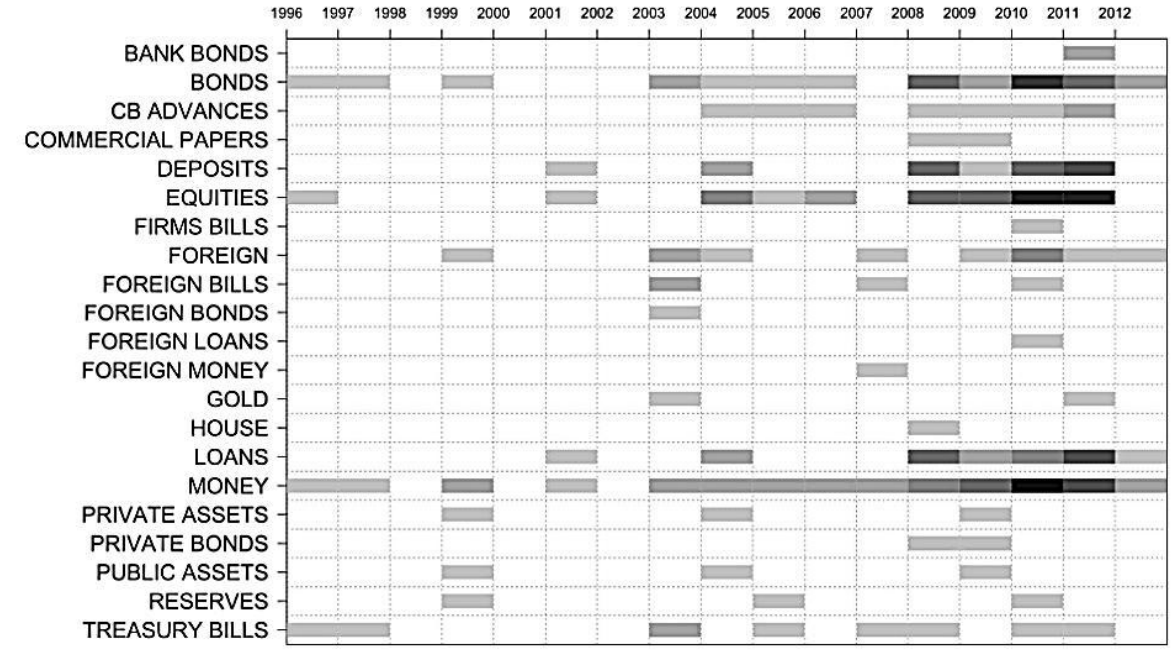
\includegraphics[width = 0.9\textwidth]{../../Escrita_Dissertacao/Da_Silveira_Dissertacao_Atual/Modelo/Caverzassi_Heatmap.png}
	\caption*{\textbf{Fonte:} \textcite[p.~4]{caverzasi_stock-flow_2013}}
\end{figure}

As etapas contábeis da abordagem SFC constituem em\footnote{Esta seção não pretende expor a metodologia pormenorizadamente, mas sim expor seus procedimentos de modo a esclarecer as etapas que foram adotadas. Para uma apresentação mais gradual, ver \textcite[Capítulo 4]{da_silveira_politica_2017}.}: (i) seleção dos setores institucionais e dos ativos a serem incorporados; (ii) mapeamento das relações dos fluxos entre os mencionados setores por meio da construção da matriz de fluxos; (iii) construção da matriz dos estoques de riqueza (real e financeira) em que são contabilizadas os ativos e passivos  bem como a posição líquida de cada setor; (iv) identificação das formas que os fluxos são financiados e sua respectiva acumulação/alocação dos estoques. Portanto, ao partir de um aparato analítico baseado em identidades macroeconômicas, surgem restrições que precisam ser seguidas.
%Vale destacar que as identidades contábeis são o ponto de partida, mas não são suficientes para garantir a consistência do modelo\footnote{Exemplo disso pode ser visto na exposição de  \textcite[p.~27--8]{godley_monetary_2007}  a despeito da contabilização das ações que não são, legalmente, um passivo das firmas e, portanto, o pagamento de dividendos não é uma obrigação contratual. Apesar disso, considera-se que as ações emitidas pelas firmas são similares aos \textit{corporate bonds}, garantindo a consistência do modelo. O que pretende ser destacado é que por mais que tal simplificação seja razoável, não deixa de ser uma hipótese.}. Para isso, é necessário que a soma da posição financeira líquida de cada setor institucional seja zero de modo que não existam ``buracos negros''. 
Tal procedimento garante que para que um setor acumule riqueza financeira, outro precisa necessariamente liquidá-la de modo que não existam ``buracos negros''.

Por mais que esta etapa é centrada nas contas nacionais, isso não implica que não possua um componente teórico associado. \textcite[p.~15--16]{macedo_e_silva_peering_2011}  pontuam que estão presentes elementos pós-keynesianos: 
(i) os agentes econômicos são categorizados de acordo com o estoque de riqueza; 
(ii) os agentes celebram contratos que impactam sua riqueza e geram fluxos monetários e implicam em mudanças na composição patrimonial desses agentes; 
(iii) ganhos e perdas de capital afetam o valor dos estoques e a dinâmica do sistema; 
(iv) a composição patrimonial dos setores institucionais evolui de forma assimétrica de acordo com o grau de alavancagem, preferência pela liquidez/risco e 
(v) o acúmulo de ativos e passivos pelos agentes interfere na correlação de forças da economia. 

Desse modo, por mais que a estrutura contábil parta das identidades, isso não a isenta de teoria. No entanto, por se tratar de identidades, nada de causal pode ser extraído delas. As relações de causalidade do modelo (agora modelo e não metodologia) decorrem das equações comportamentais que, respeitando a consistência, podem ser de qualquer linhagem teórica. Feitas essas ressalvas, dada a estrutura contábil e explicitadas as hipóteses (via equações comportamentais), resta seguir para a resolução do modelo. Como pontuam \textcite{caverzasi_stock-flow_2013}, existem duas vias: (i) simulação e (ii) descrição. A primeira delas permite expor de forma mais clara as relações entre as variáveis de modelos mais complexos em que a solução analítica não é facilmente encontrada. No entanto, tal caminho fez com que o grau de complexidade dos modelos simulados fosse exponencializada de modo que a intuição econômica torna-se facilmente turva. Diante destas complicações, a presente investigação priorizará a parcimônia de modo que serão incluídos apenas os elementos estritamente necessários para a narrativa. A justificativa desta postura decorre da maior clareza obtida sem necessariamente incorrer em um menor realismo. 

RESULTADOS ESPERADOS
\section{Cronograma das atividades}\label{cronograma}

A tabela \ref{crono} apresenta um esboço das atividades a serem desempenhadas ao longo desta pesquisa. Tendo em vista que a eventual aprovação ocorrerá quando o programa de mestrado do candidato estiver em andamento, foram destacadas em cinza as atividades que já foram desempenhadas pelo requerente. Além disso, foram destacadas em amarelo as atividades que serão executadas ao longo do período de avaliação de projetos (73 dias em média\footnote{Informação baseada no ano de 2017 e obtida no link \url{http://www.fapesp.br/estatisticas/analise/} acessado em 5 de julho de 2018}). 
Dessa forma, as células em azul correspondem às atividades a serem desenvolvidas ao longo do tempo de vigência da bolsa de auxílio. Por fim, como a dissertação será desenvolvida junto das obrigações institucionais do programa de Mestrado, optou-se por incluir uma linha referente aos créditos das disciplinas que serão cursadas. 
Dito isso, segue abaixo o cronograma mencionado:

\begin{table}[H]
	\centering
	\caption{Cronograma de atividades}
	\label{crono}
	\resizebox{\textwidth}{!}{%
		\begin{tabular}{ll|l|l|l|l|l|l|l}
			\hline\hline
			\multicolumn{1}{c}{} & \multicolumn{8}{c}{Período} \\ \cline{2-9} 
			\multicolumn{1}{c}{\multirow{-2}{*}{Atividade}} & \multicolumn{1}{c|}{0-3} & \multicolumn{1}{c|}{3-6} & \multicolumn{1}{c|}{6-9 (Avaliação)} & \multicolumn{1}{c|}{9-12} & \multicolumn{1}{c|}{12-15} & \multicolumn{1}{c|}{15-18} & \multicolumn{1}{c|}{18-21} & \multicolumn{1}{c}{21-24} \\ \hline
			\textbf{1. Fundamentação teórica} &  \multicolumn{8}{c}{}\\ \hline
			1.1. Disciplinas &  \cellcolor[HTML]{9B9B9B} & \cellcolor[HTML]{9B9B9B} & \cellcolor[HTML]{f4df09}  & \cellcolor[HTML]{5076B0}  &\cellcolor[HTML]{5076B0}  & \cellcolor[HTML]{5076B0} &  &  \\ \hline
			1.2. Revisão bibliográfica & \cellcolor[HTML]{9B9B9B} &\cellcolor[HTML]{9B9B9B}  &\cellcolor[HTML]{f4df09}  & \cellcolor[HTML]{5076B0} & \cellcolor[HTML]{5076B0} &  &  &  \\ \hline
			\textbf{2. Análise computacional} &  \multicolumn{8}{c}{}  \\ \hline
			2.1. Pesquisa em linguagem de programação   & \cellcolor[HTML]{9B9B9B} & \cellcolor[HTML]{9B9B9B} & \cellcolor[HTML]{f4df09} & \cellcolor[HTML]{5076B0} & \cellcolor[HTML]{5076B0} &  &  &  \\ \hline
			2.2. Construção do modelo teórico &  &  &  & \cellcolor[HTML]{5076B0} & \cellcolor[HTML]{5076B0} & \cellcolor[HTML]{5076B0} &  &  \\ \hline			
			\textbf{3. Análise empírica} &  \multicolumn{8}{c}{}  \\ \hline
			3.1. Coleta de dados & \cellcolor[HTML]{9B9B9B} & \cellcolor[HTML]{9B9B9B} & \cellcolor[HTML]{f4df09} & \cellcolor[HTML]{5076B0} &  &  &  &  \\ \hline
			3.2. Simulações &  &  &  &  &  & \cellcolor[HTML]{5076B0} & \cellcolor[HTML]{5076B0} &  \\ \hline
			\textbf{4. Análise dos resultados} &  \multicolumn{8}{c}{}  \\ \hline
			4.1. Comparações com a literatura &  &  &  &  &  & \cellcolor[HTML]{5076B0} & \cellcolor[HTML]{5076B0} &  \\ \hline
			4.2. Descrição dos resultados obtidos &  &  &  &  &  & \cellcolor[HTML]{5076B0} & \cellcolor[HTML]{5076B0} &  \\ \hline
			\textbf{5. Exame de qualificação} &  &  &  &  &  &  & \cellcolor[HTML]{5076B0} &  \\ \hline
			\textbf{6. Redação da Dissertação de Mestrado} &  \multicolumn{8}{c}{}  \\ \hline
			6.1. Capítulo teórico &  &  &  & \cellcolor[HTML]{5076B0} & &  &  &  \\ \hline
			6.2. Capítulo descritivo &  &  &  &  & \cellcolor[HTML]{5076B0} & \cellcolor[HTML]{5076B0} &  &  \\ \hline
			6.3. Capítulo analítico &  &  &  &  & & \cellcolor[HTML]{5076B0} & \cellcolor[HTML]{5076B0} &  \\ \hline
			\textbf{7. Defesa} &  &  &  &  &  &  &  & \cellcolor[HTML]{5076B0} \\ \hline \hline
		\end{tabular}%
	}
\end{table}


Além disso, é importante realçar que as simulações computacionais tal como pretendidas neste projeto não constam na grade regular das disciplinas recomendadas e disponíveis ao Instituto de Economia. Sendo assim, foi explicitada na tabela \ref{crono} uma linha referente ao tempo destinado ao aprendizado de linguagem de computação para obtenção dos instrumentos necessários. Dessa forma, dada a versatilidade e aceitação na academia, serão estudadas rotinas de programação em python\footnote{No momento em que este projeto está sendo elaborado, e tal como sugerido pela tabela \ref{crono}, as pesquisas em linguagem de programação estão em andamento. Neste caso, dada a familiaridade do requerente com a linguagem R, estão sendo cursados aulas de Python específicas para usuários de R disponíveis na plataforma DATACAMP. Mais informações em \url{https://www.datacamp.com/courses/python-for-r-users}, acessado em 5 de julho de 2018}. A escolha desta linhagem em particular se justifica pela estrutura gramatical de alto nível que facilita o aprendizado de seu usuário\footnote{Site oficial da linguagem python: \url{https://www.python.org}, acessado em 5 de julho de 2018}.

Desse modo, foram apresentados tantos os objetivos desta pesquisa quanto os métodos e procedimentos para concebê-la. Isso posto, a seção \ref{Result} irá apresentar os resultados esperados com esta pesquisa.
Por fim, a seção \ref{relev} tem o propósito de realçar alguns componentes relevantes deste projeto até então não mencionados.

\begin{comment}
%==========================================================
%				Descartado
%==========================================================
% Please add the following required packages to your document preamble:
% \usepackage{multirow}
% \usepackage{graphicx}
%\begin{table}[htb]
%	\centering
%	\caption{Cronograma de atividades}
%	\label{crono}
%	\resizebox{\textwidth}{!}{%
%		\begin{tabular}{|l|l|l|l|l|l|l|l|l|}
%			\hline
%			\multicolumn{1}{|c|}{} & \multicolumn{8}{c|}{Período} \\ \cline{2-9} 
%			\multicolumn{1}{|c|}{\multirow{-2}{*}{Atividade}} & \multicolumn{1}{c|}{0-3} & \multicolumn{1}{c|}{3-6} & \multicolumn{1}{c|}{6-9} & \multicolumn{1}{c|}{9-12} & \multicolumn{1}{c|}{12-15} & \multicolumn{1}{c|}{15-18} & \multicolumn{1}{c|}{18-21} & \multicolumn{1}{c|}{21-24} \\ \hline
%			\textbf{1. Fundamentação teórica} &\cellcolor[HTML]{FE0000}  & \cellcolor[HTML]{FE0000} & \cellcolor[HTML]{FE0000} & \cellcolor[HTML]{FE0000} & \cellcolor[HTML]{FE0000} & \cellcolor[HTML]{FE0000} & \cellcolor[HTML]{FE0000} &  \\ \hline
%			1.1. Disciplinas &  \cellcolor[HTML]{9B9B9B} & \cellcolor[HTML]{9B9B9B} & \cellcolor[HTML]{9B9B9B}  & \cellcolor[HTML]{9B9B9B}  &\cellcolor[HTML]{9B9B9B}  & \cellcolor[HTML]{9B9B9B} &  &  \\ \hline
%			1.2. Revisão bibliográfica & \cellcolor[HTML]{9B9B9B} &\cellcolor[HTML]{9B9B9B}  &\cellcolor[HTML]{9B9B9B}  & \cellcolor[HTML]{9B9B9B} &  &  &  &  \\ \hline
%			\textbf{2. Análise computacional} & \cellcolor[HTML]{FE0000} & \cellcolor[HTML]{FE0000} & \cellcolor[HTML]{FE0000} & \cellcolor[HTML]{FE0000} & \cellcolor[HTML]{FE0000} &\cellcolor[HTML]{FE0000}  &  &  \\ \hline
%			2.1. Pesquisa em linguagem de programação   & \cellcolor[HTML]{9B9B9B} & \cellcolor[HTML]{9B9B9B} & \cellcolor[HTML]{9B9B9B} & \cellcolor[HTML]{9B9B9B} & \cellcolor[HTML]{9B9B9B} &  &  &  \\ \hline
%			2.2. Construção do modelo teórico &  &  &  & \cellcolor[HTML]{9B9B9B} & \cellcolor[HTML]{9B9B9B} & \cellcolor[HTML]{9B9B9B} &  &  \\ \hline			
%			\textbf{3. Análise empírica} &  &  &  &  & \cellcolor[HTML]{FE0000} & \cellcolor[HTML]{FE0000} & \cellcolor[HTML]{FE0000} &  \\ \hline
%			3.1. Coleta de dados &  &  &  &  & \cellcolor[HTML]{9B9B9B} & \cellcolor[HTML]{9B9B9B} &  &  \\ \hline
%			3.2. Simulações &  &  &  &  &  & \cellcolor[HTML]{9B9B9B} & \cellcolor[HTML]{9B9B9B} &  \\ \hline
%			\textbf{4. Análise dos resultados} &  &  &  &  &  &\cellcolor[HTML]{FE0000}  & \cellcolor[HTML]{FE0000} &  \\ \hline
%			4.1. Comparações com a literatura &  &  &  &  &  & \cellcolor[HTML]{9B9B9B} & \cellcolor[HTML]{9B9B9B} &  \\ \hline
%			4.2. Descrição dos resultados obtidos &  &  &  &  &  &  & \cellcolor[HTML]{9B9B9B} &  \\ \hline
%			\textbf{5. Exame de qualificação} &  &  &  &  &  &  & \cellcolor[HTML]{009901} &  \\ \hline
%			\textbf{6. Redação da Dissertação de Mestrado} &  &  &  &  & \cellcolor[HTML]{FE0000} & \cellcolor[HTML]{FE0000} & \cellcolor[HTML]{FE0000} &  \\ \hline
%			\textbf{7. Defesa} &  &  &  &  &  &  &  & \cellcolor[HTML]{009901} \\ \hline
%		\end{tabular}%
%	}
%\end{table}





%O cronograma \ref{crono} também mostra os grupos de atividades a serem desempenhadas, são elas: (i) fundamentação teórica; (ii) Análise computacional; (iii) Análise empírica e (iv) Redação da dissertação de mestrado. O tempo previsto para a dedicação deste grupo de atividades está destacado em vermelho. Os retângulos verdes, por sua vez, representam as obrigações institucionais: (i) Exame de Qualificação e (ii) Defesa da dissertação.

\end{comment}





\section{Resultados esperados}\label{Result}
Realizada esta pesquisa, esperam-se os seguintes resultados:
\begin{itemize}
	\item As mudanças redistributivas observadas são relevantes para explicar a dinâmica da economia brasileira no período em questão;
	\item O crédito ao consumidor teve efeitos significativos tanto sobre o consumo de bens duráveis quanto no aumento do endividamento das famílias;
	\item O maior acesso ao crédito decorre tanto da maior participação dos salários na renda viabilizada pelas valorizações reais do salário mínimo (aumento do colateral) quanto medidas deliberadas de política econômica;
	\item Encontrar uma taxa de juros relevante ao longo prazo tal como argumentado por \textcite{pivetti_essay_1992};
	\item Espera-se destacar o conflito distributivo por meio de mudanças na taxa de juros mencionada acima para o caso brasileiro;
	\item Os componentes que explicam a dinâmica econômica do Brasil podem ser captados pelo modelo do supermultiplicador sraffiano.
\end{itemize}
\begin{comment}
%====================================================================================
% 							DESCARTADO
%====================================================================================
\section{Rotinas de programação em economia}

Em economia, é comum o uso de \textit{softwares} dedicados à determinadas tarefas acadêmicas. No entanto, cada vez mais são utilizadas linguagens de programação nas mais diferentes áreas de conhecimento. O desenvolvimento de rotinas de programação possibilita uma maior autonomia do pesquisador para resolver problemas específicos e assim avançar na linha de pesquisa. Além disso, a distribuição dos programas criados pode contribuir para o avanço de outras fronteiras de pesquisa de forma mais difusa.

% Desse modo,  ao desenvolver um modelo macrodinâmico partindo de uma linguagem de programação, esse projeto de pesquisa pode auxiliar mais pesquisadores em suas investigações. Neste caso, optou-se por uma linguagem voltada para \textit{data science}: R \cite{RSoftware}. Vale notar que também é uma linguagem apropriada para  análise estatística e, portanto,  de grande valia para estudos na área de economia.
\end{comment}


\begin{comment}
%====================================================================================
% 							TÓPICOS RELEVANTES
%====================================================================================
% Interdisciplinaridade
% Simulação
% Avanço na fronteira heterodoxa
\end{comment}

%====================================================================================
% 							INÍCIO
%====================================================================================


%{\let\clearpage\relax \chapter{Elementos relevantes do projeto}\label{relev}}
{\let\clearpage\relax \chapter{Contribuição dos resultados}\label{relev}}

\section{Interdisciplinariedade}
O objeto de análise deste projeto conta com elementos que não se limitam à ciência econômica. Desse modo, cabe ao pesquisador não apenas ficar circunscrito à sua área de interesse como também ser capaz de captar interpretações das outras áreas do conhecimento. O capítulo descritivo apresentado na seção \ref{Metodo} possui tal característica. O uso de elementos explicativos trazidos da sociologia tal como o conceito de cultura do consumo \cites{isleide_a._fontenelle_alcances_2016}{streeck_citizens_nodate} possibilitam o rompimento da insularidade das ciências econômicas. Sendo assim, o devido uso da interdisciplinariedade tem um caráter enriquecedor que pode ser melhor explorado por estudos futuros.

\section{Simulação Computacional e reprodutibilidade}
%TODO Revisar: 06/07
Como apresentado na seção \ref{Metodo}, esta pesquisa fará uso de simulações computacionais para analisar as implicações do modelo teórico proposto. O uso de tal ferramenta permite não apenas a verificação das discussões apresentadas pela literatura como também a reprodutibilidade dos resultados. Tendo em vista essas possibilidades, o presente projeto irá disponibilizar as rotinas de programação utilizadas. Com isso, é facilitada tanto a revisão por pares quanto a divulgação dos métodos utilizados. Além disso, a distribuição dos dados e códigos permite que o avanço científico não fique restrito às instituições de pesquisas com maior aporte financeiro. Por fim, para que esse propósito seja viabilizado, será utilizada uma plataforma de código livre \cite{center_for_open_science_osfhome_nodate}.

\section{Avanço na fronteira de pesquisa heterodoxa}

Por estar na fronteira de pesquisa, abordagem do supermultiplicador sraffiano está em constante mudança. Não apenas isso, mas pesquisas recentes que utilizam este modelos não estão restritas à abordagem do excedente. A inclusão deste modelo pela escola Pós-Keynesiana por meio da metodologia \textit{Stock-Flow Consistent} tal como em \textcite{brochier_endogenous_2018}
permite que avanços aqui realizados se estendam para as escolas de pensamento não-ortodoxas como um todo. Nesses termos, a relevância do presente projeto se dá também pelo aprimoramento e avanço da fronteira de pesquisa heterodoxa.






\endgroup
%=====================================================================
% 							Bibliografia
%=====================================================================
%{\let\clearpage\relax \chapter{Bibliografia}}
%-----

\section*{Bibliografia}

{\let\clearpage\relax\printbibliography[title = {Referências Bibliográficas}]}


%=====================================================================
% 							Fim do Documento
%=====================================================================
\end{document}